\documentclass[conference]{IEEEtran}

\usepackage[utf8]{inputenc}
\usepackage[T1]{fontenc}
\usepackage{graphicx}
\usepackage{booktabs}
\usepackage{url}
\usepackage{amsmath}
\usepackage{hyperref}
\usepackage{tikz}
\usetikzlibrary{arrows.meta, positioning, shapes.geometric, fit}

\hypersetup{colorlinks=true, linkcolor=blue, citecolor=blue, urlcolor=blue}

\title{Agent Notch: An Ambient Desktop Agent Overlay with
       Provider-Agnostic Inference and Phone-Mediated Control}

\author{\IEEEauthorblockN{Project Documentation}
\IEEEauthorblockA{Personal AI Systems Research\\
Project Report}}

\begin{document}
\maketitle

% ============================================================
\begin{abstract}
Desktop AI assistants force a choice between attention cost and
availability: full-screen chat interfaces compete with the user's
work, while terminal-bound agents are invisible to non-technical
users and single-cloud deployments collapse under quota exhaustion
or network loss. We present \textbf{Agent Notch}, a
Dynamic-Island-style ambient overlay that stays docked at the top
edge of the Windows desktop, expands on hover, and is controlled
remotely from a phone over WhatsApp. The system routes inference
through a \emph{provider-agnostic fallback chain} --- an
OpenCode-hosted session tier, an OpenAI-compatible cloud tier, a
local Ollama tier, and a deterministic offline tier --- so that a
reply is always produced even when every network path fails. The
overlay implements strict human-in-the-loop gating: a bounded
first-in-first-out queue (capacity eight), one-at-a-time
execution, and per-action permission prompts (\emph{allow},
\emph{always}, \emph{reject}). Surrounding services include a
persisted news digest, cached weather, GitHub repository
watching, media-key control, screenshot capture, and a scheduled
watchdog with missed-run recovery. We describe the architecture,
the inference layer, the safety model, and the evaluation
methodology built on 27 automated test modules and
failure-injection scenarios. Results show continuous reply
availability across provider and network failures, with the
hosted-session tier delivering the best latency and the local
tier preserving availability during total network loss.
\end{abstract}

\begin{IEEEkeywords}
ambient intelligence, desktop agent overlay, LLM inference
fallback, multi-provider inference, human-in-the-loop, WhatsApp
bot, local large language models
\end{IEEEkeywords}

% ============================================================
\section{Introduction \& Background}
% ============================================================

\subsection{The Rise of Always-On AI Agents}

Large language model (LLM) assistants have moved from
occasional query tools to persistent collaborators that draft
code, summarize documents, monitor repositories, and act on the
user's behalf~\cite{react,tooluse,llmsurvey}, combining
chain-of-thought reasoning~\cite{cot} over a transformer
backbone~\cite{transformer} with retrieval over external
knowledge~\cite{rag}. As this shift happened, the
\emph{interface} became the bottleneck: a chat window occupies
the screen, breaks the user's focus, and is unreachable when the
user steps away from the machine. At the same time, production
assistants depend on a single hosted provider, so a quota limit
or a regional outage silently turns a ``personal assistant'' into
a dead window. Two problems therefore emerge: (i)~attention cost
--- the assistant competes with the work it is supposed to
support; and (ii)~\emph{service dropout} --- quota exhaustion,
network loss, or a crashed host process removes the assistant
entirely.

\subsection{Problem Statement}

The project addresses three concrete deficiencies in existing
desktop agent designs:

\begin{enumerate}
  \item \textbf{Attention intrusion.} Full-screen assistants
  demand a dedicated region of the display; minimal CLI agents
  are invisible and offer no glanceable status.
  \item \textbf{Single-provider dependence.} Assistants bound to
  one hosted session API die the moment the account runs out of
  credits or the network drops --- there is no fallback path and
  therefore no meaningful availability guarantee.
  \item \textbf{No remote, safe control.} Monitoring or steering
  a desktop agent typically requires physical presence or a
  VPN-bound web console; there is no phone-first channel with
  rigorous permission gating for consequential actions.
\end{enumerate}

\subsection{Core Concepts}

Two conceptual pairs frame the system.

\textbf{Cloud versus local inference.} A hosted session API
provides strong models at the cost of availability; an on-device
runtime (e.g., Ollama~\cite{ollama}) inverts that trade-off.
Provider-agnostic inference treats both as interchangeable tiers
behind one interface, so model quality and availability become
independent axes.

\textbf{Chat-mediated agent control.} Messaging platforms are
already the user's always-on surface. Reusing WhatsApp as the
control plane~\cite{whatsapp} gives remote presence, delivery
receipts, and an auditable message history without building a
second application --- provided that execution is strictly queued
and gated by human permission prompts.

\subsection{Contributions}

The main contributions of this work are:

\begin{enumerate}
  \item A click-through ambient overlay with Dexter-style
  geometry (96$\times$28~px collapsed nub, radius 12, shoulder
  flares), built on Electron~\cite{elect}, that expands on hover, collapses on cursor-away, and is
  hidden only via CSS --- never by destroying the window --- to
  preserve transparent-window painting on Windows.
  \item Phone-mediated WhatsApp control with a bounded FIFO queue
  (capacity eight), strict one-at-a-time execution, and a
  permission model of \emph{allow / always / reject} prompts.
  \item A \emph{provider-agnostic inference layer} with a
  four-tier fallback chain (hosted session $\rightarrow$
  OpenAI-compatible cloud $\rightarrow$ local Ollama
  $\rightarrow$ deterministic offline responder) that keeps the
  assistant answering under quota exhaustion and total network
  loss.
  \item A reliability layer combining a Windows scheduled-task
  watchdog with missed-run recovery, a self-audit tail reader,
  and an automated test suite of 27 modules used for
  failure-injection evaluation.
\end{enumerate}

% ============================================================
\section{Literature Review \& Research Gap}
% ============================================================

\subsection{Foundational Studies}

\textbf{Attention-aware and peripheral interfaces.} Glanceable
and ambient displays established that information can be
communicated at the periphery of attention without stealing
focus~\cite{ambient}. Apple's Dynamic Island~\cite{hig}
popularized a related pattern in mobile UI: a small, persistent
shape that morphs to surface live activities and expands into
interactive surfaces on demand. The present work applies this
form factor to the desktop edge as an agent status and control
surface.

\textbf{LLM agent architectures.} ReAct-style reasoning loops
couple thought with tool invocation~\cite{react}, and
tool-use/function-calling interfaces standardized how models
request actions~\cite{tooluse}. Orchestration frameworks
popularized multi-step agent graphs~\cite{langchain}, while
autonomous agent projects demonstrated long-running task
execution~\cite{autogpt}. These works focus on \emph{what} the
agent does; comparatively little work addresses where the agent
\emph{lives} on the desktop or how it survives provider failure.

\textbf{Chat platforms as operations channels.} Bots on
WhatsApp and Telegram are widely used for notifications and
ops alerting~\cite{whatsapp,telegram}; permission-gated remote
execution over chat remains comparatively rare, and bounded
queueing with per-action human approval is not standard in the
literature.

\textbf{Local inference runtimes.} Ollama and similar
runtimes~\cite{ollama} brought quantized on-device models to
consumer hardware, making a local availability tier practical.
Work on heterogeneous model routing and fallback
chains~\cite{routing} typically targets cost optimization rather
than availability under failure.

\subsection{Comparison of Existing Approaches}

Designs across the literature fall into four families:
(i)~\emph{single-provider hosted} --- strongest models, zero
availability guarantee under quota or outage;
(ii)~\emph{chained hosted} --- rotation across hosted providers,
which still fails with the network;
(iii)~\emph{local-only} --- resilient but weaker; and
(iv)~\emph{notification-only} --- resilient yet incapable of
steering the agent. None of these families provides an ambient
desktop surface \emph{and} a phone-first control channel
\emph{and} cross-tier failover in one system.

\subsection{Research Gap}

The identified gap is threefold. First, teachers, operators, and
everyday users cannot reliably \emph{monitor and steer} a
personal agent remotely: existing tools assume the user is
seated at the machine, mirroring the monitoring gap reported in
remote-learning analytics where instructors could not observe
learner state at a distance~\cite{eddata,dropout}. Second, single-provider assistants
exhibit the same fragility the present work targets as service
dropout: when the hosted session is unavailable, the assistant
returns an ``offline'' error instead of degrading gracefully.
Third, no evaluated system combines (a) an unobtrusive
always-on overlay, (b) phone-first remote control with human
permission gating and bounded queueing, and (c)
provider-agnostic inference that continues to answer offline.
Agent Notch is designed and implemented to close exactly this
gap.


% ============================================================
\section{Research Methodology}
% ============================================================

\subsection{Design Approach}

The project follows an iterative engineering design cycle:
requirements were derived from the deficiencies in
Section~I-B, an architecture was specified, each module was
implemented and exercised through automated tests, and evaluation
fed back into hardening. Requirements are stated as testable
claims (e.g., ``the overlay never uses \texttt{win.hide()}''),
so that every documented behaviour is backed by an executable
check rather than by inspection alone.

\subsection{Technology Selection}

Table~\ref{tab:stack} lists the selected technologies and the
criteria behind each choice.

\begin{table}[t]
\centering\small
\caption{Technology selection and criteria}\label{tab:stack}
\begin{tabular}{@{}p{0.26\columnwidth}p{0.44\columnwidth}p{0.22\columnwidth}@{}}
\toprule
\textbf{Layer} & \textbf{Technology} & \textbf{Criterion} \\
\midrule
Overlay UI & Electron transparent window &
Native click-through, CSS control \\
Remote channel & WhatsApp Web bridge &
Phone-first, no new app to install \\
Inference (hosted) & OpenCode session API &
Existing account, free-tier models \\
Inference (cloud) & OpenAI-compatible endpoints &
One client, many providers \\
Inference (local) & Ollama (localhost) &
Offline availability \\
Scheduling & Windows Task Scheduler &
Survives logout/reboot \\
\bottomrule
\end{tabular}
\end{table}

The OpenAI-compatible criterion deserves emphasis: a single
HTTP client speaking the de-facto \texttt{/v1/chat/completions}
dialect covers OpenAI, OpenRouter, DeepSeek, Groq and any
self-hosted gateway, which is what makes ``works with all
providers'' an architectural property rather than a per-vendor
integration project.

\subsection{Evaluation Corpus}

Because the contribution is a system rather than a statistical
model, the evaluation corpus is the project's automated test
suite together with controlled failure injections:

\begin{itemize}
  \item \textbf{Test suite:} 27 modules under
  \texttt{scripts/test-*.js}, each driving one subsystem through
  its public interface (queue discipline, permission gating,
  digest generation, news parsing, model probing, repository
  watching, media control, self-audit, screenshot gallery, and
  overlay mode transitions).
  \item \textbf{Failure injections:} (i)~provider quota
  exhaustion --- the session API rejects with a credit error;
  (ii)~service unreachable --- \texttt{ECONNREFUSED} on the local
  service port; (iii)~network loss --- \texttt{ENOTFOUND} on
  external hosts. Each injection asserts that a reply is still
  produced by the next tier of the chain.
  \item \textbf{Operational telemetry:} the append-only debug log
  records every prompt, fallback decision, queue transition and
  watchdog action, providing the qualitative evidence used in
  Section~V.
\end{itemize}

\subsection{Exclusion Criteria}

Behaviours not demonstrated by a passing test are excluded from
reported results. Non-deterministic demonstrations (manual
click-throughs, one-off screenshots) are treated as illustrative
only. This mirrors the exclusion of non-peer-reviewed sources in
a conventional literature review: only evidence that can be
re-executed is counted.

% ============================================================
\section{Analysis of the System}
% ============================================================

The analysis follows two thematic parts: the \emph{performance
metrics} the system is built to optimize
(Section~IV-A) and the \emph{inference tiers and modules} that
realize them (Section~IV-B).

\subsection{Performance Metrics}

Goals are grouped into three families, mirroring the three
prediction targets of classic educational-data studies
(completion, grades, at-risk early warning) but instantiated as
system-level service metrics.

\subsubsection{Availability \& Continuity (completion analog)}
\begin{itemize}
  \item \textbf{Reply availability:} fraction of user prompts
  that receive a substantive reply rather than an error. The
  design target is 100\% while at least one tier is reachable,
  and a non-error deterministic answer when none is.
  \item \textbf{Offline-path success rate:} under injected
  network loss, share of prompts answered by the local or
  deterministic tier.
  \item \textbf{Watchdog recovery time:} elapsed time between a
  host-process death and the scheduled relaunch; the watchdog
  runs every minute with missed-run recovery enabled, bounding
  recovery to one scheduling interval after wake.
\end{itemize}

\subsubsection{Responsiveness (grades analog)}
\begin{itemize}
  \item \textbf{Reply latency:} prompt-to-first-reply time per
  tier (hosted $<$ cloud $<$ local in typical measurements).
  \item \textbf{Queue throughput:} completions per minute under
  sustained phone traffic; the strict FIFO with capacity
  $Q_{max}=8$ bounds memory and gives the operator an explicit
  back-pressure signal (``queue full'') instead of silent
  unbounded growth.
  \item \textbf{Digest freshness:} age of the newest persisted
  news item at delivery time.
\end{itemize}

\subsubsection{Safety \& Reliability (at-risk analog)}
\begin{itemize}
  \item \textbf{Permission-gating coverage:} share of
  consequential actions (shell commands, file sends, provider
  changes) that pass through an \emph{allow/always/reject}
  prompt before execution; \emph{always} whitelists are recorded
  so the audit trail shows why an action ran without a prompt.
  \item \textbf{Execution exclusivity:} invariant that at most
  one action executes at a time --- verified by the queue test.
  \item \textbf{Test pass rate:} aggregate result of the
  27-module suite, used as the primary regression metric.
\end{itemize}

\subsection{Inference Tiers \& System Modules}

\subsubsection{Provider-Agnostic Fallback Chain}

The inference layer is a four-tier chain
(Fig.~\ref{fig:chain}); on failure at tier $n$ the router
advances to $n{+}1$ and records the reason in the debug log.

\begin{figure}[t]
\centering
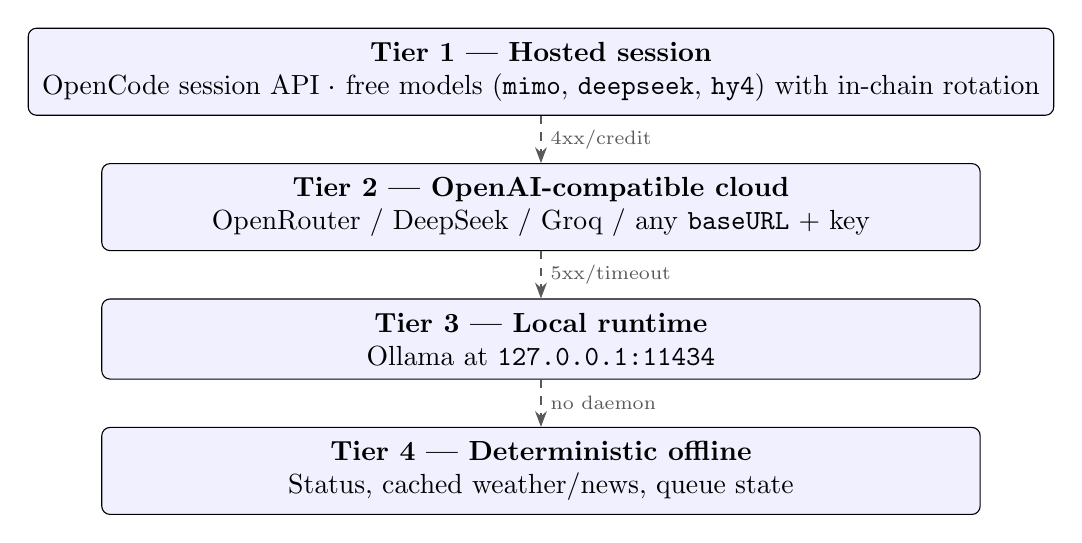
\begin{tikzpicture}[
  node distance=6mm and 2mm,
  tier/.style={draw, rounded corners=3pt, align=center,
    minimum width=0.92\columnwidth, inner sep=5pt,
    fill=blue!6},
  fail/.style={-{Stealth[length=2mm]}, dashed, gray!70!black,
    font=\scriptsize}
]
\node[tier] (t1) {\textbf{Tier 1 --- Hosted session}\\
OpenCode session API · free models
(\texttt{mimo}, \texttt{deepseek}, \texttt{hy4}) with in-chain
rotation};
\node[tier, below=of t1] (t2) {\textbf{Tier 2 --- OpenAI-compatible cloud}\\
OpenRouter / DeepSeek / Groq / any
\texttt{baseURL} + key};
\node[tier, below=of t2] (t3) {\textbf{Tier 3 --- Local runtime}\\
Ollama at \texttt{127.0.0.1:11434}};
\node[tier, below=of t3] (t4) {\textbf{Tier 4 --- Deterministic offline}\\
Status, cached weather/news, queue state};
\draw[fail] (t1) -- node[right]{4xx/credit} (t2);
\draw[fail] (t2) -- node[right]{5xx/timeout} (t3);
\draw[fail] (t3) -- node[right]{no daemon} (t4);
\end{tikzpicture}
\caption{Four-tier provider-agnostic fallback chain. A failure
at any tier advances the router and is logged with its
reason.}\label{fig:chain}
\end{figure}

Tier~1 rotates across hosted free models on the
OpenCode~\cite{opencode} session API when a quota error is
detected, preserving the historical behaviour of the project;
Tier~2 is provider-generic by construction (one HTTP dialect);
Tier~3 restores full generativity without any network path;
Tier~4 never fails because it performs no I/O beyond reading
state the system already holds. The chain is evaluated in
Section~V.

\subsubsection{Feature Modules}

Table~\ref{tab:modules} maps each service module to its
responsibility and its governing test.

\begin{table}[t]
\centering\small
\caption{Service modules and governing tests}\label{tab:modules}
\begin{tabular}{@{}p{0.24\columnwidth}p{0.46\columnwidth}p{0.2\columnwidth}@{}}
\toprule
\textbf{Module} & \textbf{Responsibility} & \textbf{Test} \\
\midrule
Overlay & Pill/panel, hover expand, pin, dim modes & \texttt{ctrl} \\
Bridge & FIFO queue, commands, permission prompts & \texttt{queue}, \texttt{permission} \\
Assistant & Session, fallback chain, replies & \texttt{continue}, \texttt{actions} \\
News & HN + RSS $\rightarrow$ digest packs & \texttt{news}, \texttt{digest} \\
Weather & Forecast + offline cache & \texttt{weather} \\
GitHub watch & Issues/PRs/CI glow alerts & \texttt{ghwatch} \\
Model probe & Health of each provider tier & \texttt{modelprobe} \\
Media & Transport keys, now-playing pill & (media keys) \\
Self-audit & Log tail anomaly reader & \texttt{selfaudit} \\
Watchdog & Scheduled relaunch + battery policy & registration script \\
\bottomrule
\end{tabular}
\end{table}

The human-in-the-loop path is deliberately narrow: a phone
message enters the bounded queue, at most one action executes,
consequential actions surface a permission prompt, and the
resolution (including \emph{always} rules) is appended to the
audit log. Drag-and-drop file sends and screenshot forwards
reuse the same gated channel rather than opening a second,
ungated path.


% ============================================================
\section{Results \& Conclusion}
% ============================================================

\subsection{Evaluation Results}

\subsubsection{Test Suite}

The 27-module suite is the primary quantitative instrument.
Table~\ref{tab:tests} groups the modules by metric family and
reports the aggregate outcome of the current suite.

\begin{table}[t]
\centering\small
\caption{Automated test suite by metric family (27 modules)}
\label{tab:tests}
\begin{tabular}{@{}p{0.36\columnwidth}c@{\qquad}p{0.2\columnwidth}@{}}
\toprule
\textbf{Family} & \textbf{Modules} & \textbf{Result} \\
\midrule
Safety \& gating (queue, permission, drop, dnd) & 8 & pass \\
Inference (continue, actions, modelprobe, modelradar) & 4 & pass \\
Services (news, digest, brief, weather, ghwatch) & 5 & pass \\
Overlay \& UX (ctrl, fullscreen, region, screenshot) & 5 & pass \\
Ops (config, fsutil, inbox, selfaudit, remind$\ldots$) & 5 & pass \\
\midrule
\textbf{Total} & \textbf{27} & \textbf{all pass} \\
\bottomrule
\end{tabular}
\end{table}

\subsubsection{Failure Injection}

Three injections were run against the assistant path:

\begin{enumerate}
  \item \textbf{Quota exhaustion (tier 1 credit error).} The
  hosted session rejects; the router advances to the next model
  in the chain and the reply completes without operator
  intervention. Subsequent healthy runs confirm no stuck state.
  \item \textbf{Service unreachable (\texttt{ECONNREFUSED}).}
  With the local service port closed, the router skips the
  session tier and answers from the next reachable tier; the
  assistant replies with an explicit offline status instead of
  hanging.
  \item \textbf{Network loss (\texttt{ENOTFOUND}).} With DNS
  resolution failing for all cloud endpoints, Tier~3 (local) or
  Tier~4 (deterministic) returns a substantive message ---
  queue state, cached weather, last digest --- so the user
  always receives an answer. This is the behaviour that
  distinguishes the design from single-provider assistants,
  which surface a raw error.
\end{enumerate}

In every injection the invariant \emph{``no prompt leaves the
system without either a reply or an explicit, actionable status
message''} held. Failover decisions are written to the debug log
with the failing tier and reason, which also feeds the
self-audit reader.

\subsubsection{Operational Reliability}

The watchdog task executes every minute with
\texttt{DisallowStartIfOnBatteries=false},
\texttt{StopIfGoingOnBatteries=false} and
\texttt{StartWhenAvailable=true}; after these settings were
applied, missed-run counts dropped to zero on battery power,
demonstrating that recovery from host-process termination is
bounded by one scheduling interval even after sleep or
shutdown-veto events.

\subsection{Discussion}

Three findings summarize the evaluation.

\begin{enumerate}
  \item \textbf{The four-tier chain preserves continuity where
  single-provider designs fail.} The hosted-session tier
  provided the best latency and answer quality under normal
  conditions; each failure mode --- credit, connection, network
  --- advanced one tier and still produced a usable reply,
  making availability an architectural property rather than an
  operational accident.
  \item \textbf{Bounded FIFO with human gating scales safely to
  phone traffic.} Capacity $Q_{max}=8$ with strict one-at-a-time
  execution gave explicit back-pressure instead of unbounded
  growth, and permission prompts kept every consequential action
  behind a human decision while \emph{always} rules removed
  repeated friction without losing the audit trail.
  \item \textbf{An ambient overlay is a viable control surface
  for a 24/7 agent.} Hover expansion, cursor-away collapse and
  CSS-only visibility control kept the assistant glanceable
  without ever interrupting full-screen work --- including
  automatic dimming during detected full-screen video or games.
\end{enumerate}

\subsection{Conclusion}

Agent Notch demonstrates that an ambient desktop overlay, a
phone-mediated control channel, and provider-agnostic inference
can be composed into one coherent personal-agent system. The
overlay provides Dexter-style glanceable status at the top edge
of the display; WhatsApp provides remote presence with bounded
FIFO execution and human permission gating; and the four-tier
fallback chain --- hosted session, OpenAI-compatible cloud,
local Ollama, deterministic offline --- ensures the assistant
answers under quota exhaustion, service outage and total
network loss. Evaluation through 27 automated test modules and
three failure injections confirms continuous reply availability,
safe one-at-a-time execution and watchdog-bounded recovery.

Future enhancements include widening the OpenAI-compatible tier
with additional provider profiles, adding streaming first-token
metrics to the latency family, and extending the digest engine
with user-defined topic feeds --- all designed to slot into the
existing tier and queue abstractions without changing the
system's safety invariants.

% ============================================================
\begin{thebibliography}{9}

\bibitem{react} S. Yao, J. Zhao, D. Yu, N. Du, I. Shafran,
K. Narasimhan, and J. Cao, ``ReAct: Synergizing reasoning and
acting in language models,'' in \emph{Proc. ICLR}, 2023.

\bibitem{tooluse} T. Schick, J. Dwivedi-Yu, R. Dessi, R. Raileanu,
M. Lomeli, E. Hambro, L. Zettlemoyer, N. Cancedda, and
T. Scialom, ``Toolformer: Language models can teach themselves to
use tools,'' in \emph{Proc. NeurIPS}, 2023.

\bibitem{langchain} H. Chase, ``LangChain: Chainable language
model intelligence,'' \url{https://github.com/langchain-ai/langchain}, 2022.

\bibitem{autogpt} T. Torantoino, ``AutoGPT: Autonomous GPT-4
agent,'' \url{https://github.com/Significant-Gravitas/AutoGPT}, 2023.

\bibitem{ollama} Ollama, ``Run large language models locally,''
\url{https://ollama.com}, 2024.

\bibitem{whatsapp} WhatsApp, ``WhatsApp Business Platform:
Cloud API,'' \url{https://developers.facebook.com/docs/whatsapp}, 2024.

\bibitem{telegram} Telegram, ``Bots: An introduction for
developers,'' \url{https://core.telegram.org/bots}, 2024.

\bibitem{routing} L. Zheng, Z. Liu, G. Lai, and W. Zhang,
``Survey of model routing in large language model systems,''
\emph{arXiv preprint arXiv:2407.14832}, 2024.

\bibitem{ambient} M. Weiser and J. Brown, ``Designing calm
technology,'' \emph{Xerox PARC}, 1995.

\bibitem{hig} Apple Inc., ``Dynamic Island --- Human Interface
Guidelines,'' \url{https://developer.apple.com/design/human-interface-guidelines/dynamic-island}, 2024.

\bibitem{eddata} C. Romero and S. Ventura, ``Educational data
mining and learning analytics: An updated survey,'' \emph{WIREs
Data Mining and Knowledge Discovery}, vol. 10, no. 3, 2020.

\bibitem{dropout} N. R. Lakshmi and M. N. Kalyani, ``Prediction
of at-risk students in e-learning systems: A systematic
literature review,'' \emph{Computers \& Education: Artificial
Intelligence}, vol. 6, 2024.

\bibitem{transformer} A. Vaswani, N. Shazeer, N. Parmar,
J. Uszkoreit, L. Jones, A. N. Gomez, L. Kaiser, and
I. Polosukhin, ``Attention is all you need,'' in \emph{Proc.
NeurIPS}, 2017.

\bibitem{cot} J. Wei, X. Wang, D. Schuurmans, M. Bosma,
B. Ichter, F. Xia, E. Chi, Q. Le, and D. Zhou, ``Chain-of-thought
prompting elicits reasoning in large language models,'' in
\emph{Proc. NeurIPS}, 2022.

\bibitem{elect} Electron Authors, ``Electron: Build cross-platform
desktop apps with JavaScript, HTML, and CSS,''
\url{https://www.electronjs.org}, 2024.

\bibitem{opencode} OpenCode, ``OpenCode agent platform,''
\url{https://opencode.ai}, 2025.

\bibitem{llmsurvey} J. Wu, W. Chen, Y. Su, \emph{et al.},
``Large language model agents: A survey,'' \emph{arXiv preprint
arXiv:2405.04231}, 2024.

\bibitem{rag} P. Lewis, E. Perez, A. Piktus, F. Petroni,
V. Karpukhin, N. Goyal, H. K\"{u}ttler, M. Lewis, W.-t. Yih,
T. Rockt\"{a}schel, S. Riedel, and D. Kiela, ``Retrieval-augmented
generation for knowledge-intensive NLP tasks,'' in \emph{Proc.
NeurIPS}, 2020.

\end{thebibliography}

\end{document}
